\documentclass[14pt]{extarticle}
\usepackage[a4paper, left=2cm, right=2cm, top=1.5cm, bottom=2cm]{geometry}
\usepackage[utf8]{inputenc}
\usepackage[T2A]{fontenc}
\usepackage[russian]{babel}
\usepackage{indentfirst}
\usepackage{enumitem}
\usepackage{amsmath,amsfonts,amssymb}
\usepackage{icomma}
\usepackage{graphicx}
\usepackage{framed}
\usepackage{caption}
\usepackage{float}
\usepackage{titletoc}
\usepackage{hyperref}
\usepackage{paratype}
\renewcommand{\rmdefault}{PTSans-TLF}


\begin{document}
	
	\thispagestyle{empty}
	
	\begin{center}
		
		\textbf{Санкт-Петербургский политехнический университет}\\
		\vspace{2cm}
		
		Направление подготовки \\
		\large <<01.03.02 Прикладная математика и информатика>>\\
		
		\vspace{7cm}
		
		Отчет по лабораторной работе №4:\\
		\vspace{0.2cm}
		\textbf{\LARGE Решение интегралов с помощью квадратурных формул типа Гаусса}
		
		\vspace{6cm}
		
		\begin{flushleft}
			Выполнил студент гр. 5030102/40003 \hfill Т.Р. Абдуллин\\
			Преподаватель: \hfill К.Н. Козлов\\
		\end{flushleft}
		
		\vspace{3cm}
		
		Санкт-Петербург\\
		2026
	\end{center}
	
	%-------- the beginning of report --------
	
	\tableofcontents
	%-------- the first point --------
	\newpage
	\section{\Large \underline{Формулировка задачи и ее формализация}}
	Требуется разработать и реализовать численный метод вычисления определённого интеграла вида
	\[
	I = \int\limits_a^b f(x)\,dx,
	\]
	где функция $f(x)$ задаётся в виде
	\[
	f(x) = P(x)\cdot \cos(2x),
	\]
	а $P(x)$ — многочлен, заданный по варианту:
	\[
	P(x) = x^5 - 6.2x^3 + 3.5x^2 - 7x.
	\]
	
	Для вычисления интеграла необходимо использовать квадратурные формулы типа Гаусса–Лобатто с фиксированными узлами, содержащие 4 и 5 узлов.
	
	\subsection{Формализация задачи:}
	
	Рассматривается задача численного вычисления интеграла:
	\[
	I = \int\limits_a^b f(x)\,dx.
	\]
	
	Квадратурная формула Гаусса–Лобатто имеет вид:
	\[
	I \approx Q_n(f) = \frac{b-a}{2} \sum_{i=1}^{n} w_i f(x_i),
	\]
	где:
	\begin{itemize}
		\item $x_i$ — узлы квадратурной формулы на отрезке $[-1,1]$;
		\item $w_i$ — соответствующие веса;
		\item $n$ — число узлов (в данной работе $n=4,5$).
	\end{itemize}
	
	Переход к произвольному отрезку осуществляется заменой:
	\[
	x = \frac{b+a}{2} + \frac{b-a}{2} t.
	\]
	
	Точность метода обеспечивается адаптивным разбиением отрезка $[a,b]$ на $N$ частей:
	\[
	[a,b] = \bigcup_{k=1}^{N} [x_k, x_{k+1}].
	\]
	
	Критерий остановки:
	\[
	|I_{n+1} - I_n| < \varepsilon.
	\]
	
	Для повышения точности используется поправка Ричардсона:
	\[
	I^* = I_h + \frac{I_h - I_{2h}}{2^p - 1},
	\]
	где $p$ — порядок метода.
	
	%-------- the second point --------
	
	\newpage
	\section{Алгоритм метода}
	
	\subsection{Псевдокод алгоритма}
	
	\textbf{Вход:} $a, b, \varepsilon$
	
	\textbf{Выход:} приближённое значение интеграла $I$
	
	\textbf{Функция AdaptiveIntegrate($a, b, \varepsilon$):}
	
	\begin{enumerate}
		\item Вычислить интеграл на отрезке $[a,b]$:
		\[
		I_{\text{whole}} = Q_5(a,b)
		\]
		
		\item Разбить отрезок пополам:
		\[
		m = \frac{a+b}{2}
		\]
		
		\item Вычислить интегралы на подотрезках:
		\[
		I_{\text{left}} = Q_5(a,m), \quad I_{\text{right}} = Q_5(m,b)
		\]
		
		\item Найти оценку ошибки:
		\[
		\delta = |I_{\text{whole}} - (I_{\text{left}} + I_{\text{right}})|
		\]
		
		\item Если $\delta < \varepsilon$, то:
		\begin{itemize}
			\item вернуть $I = I_{\text{left}} + I_{\text{right}}$
			\item вернуть число сегментов $=1$
		\end{itemize}
		
		\item Иначе:
		\begin{itemize}
			\item рекурсивно вызвать:
			\[
			I_1 = AdaptiveIntegrate(a, m, \varepsilon/2)
			\]
			\[
			I_2 = AdaptiveIntegrate(m, b, \varepsilon/2)
			\]
			
			\item вернуть:
			\[
			I = I_1 + I_2
			\]
			\[
			N = N_1 + N_2
			\]
		\end{itemize}
		
	\end{enumerate}
	
	\subsection{Условия применимости метода}
	
	Для корректного применения квадратурных формул Гаусса–Лобатто необходимо выполнение следующих условий:
	
	\begin{itemize}
		\item функция $f(x)$ должна быть непрерывной на отрезке $[a,b]$;
		\item функция должна обладать достаточной гладкостью (наличие производных до порядка $p$);
		\item интеграл должен существовать (быть конечным);
		\item не должно быть разрывов, особенностей или сингулярностей внутри отрезка;
		\item для оценки порядка точности требуется равномерная сетка.
	\end{itemize}
	
	%-------- the third point --------
	
	\section{\Large \underline{Проверка условий применимости}}
	
	\begin{figure}[H]
		\centering
		\begin{framed}
			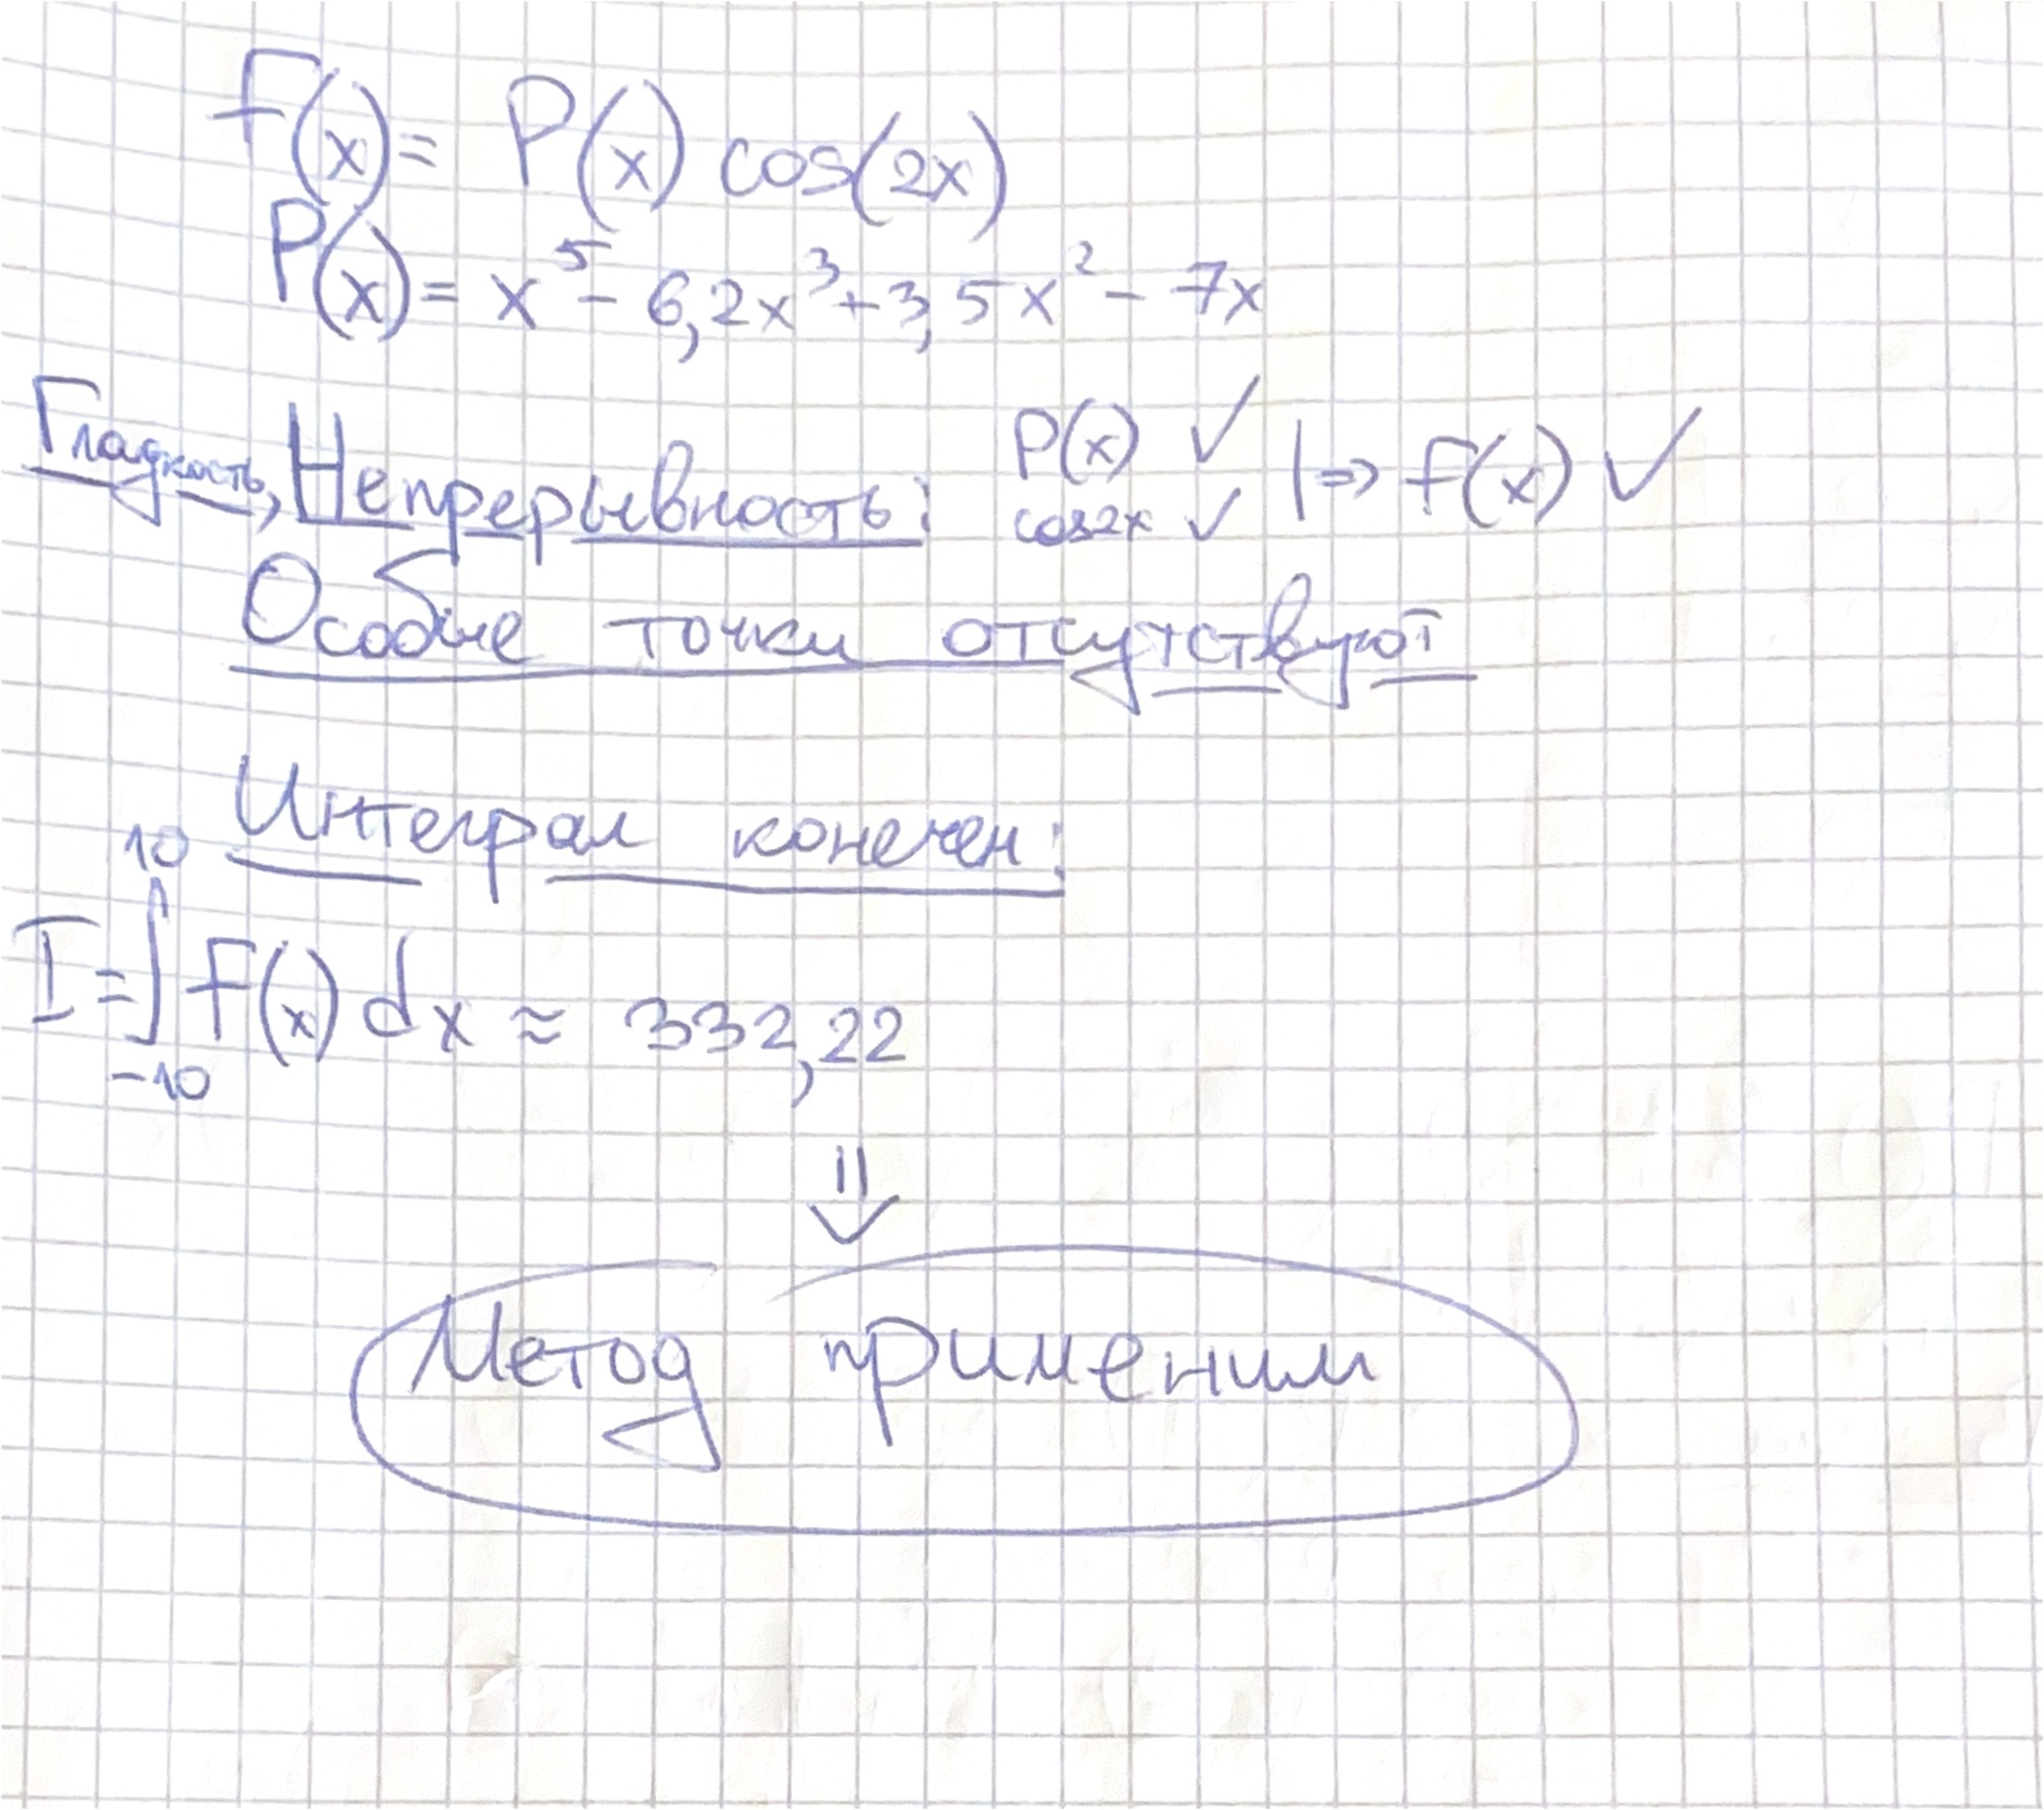
\includegraphics[width=0.9\linewidth]{../data/check.pdf}
			\caption{Проверка условий применимости}
			\label{fig:check}
		\end{framed}
	\end{figure}
	
	
	\section{\Large \underline{Предварительный анализ задачи}}
	
	\begin{figure}[H]
		\centering
		\begin{framed}
			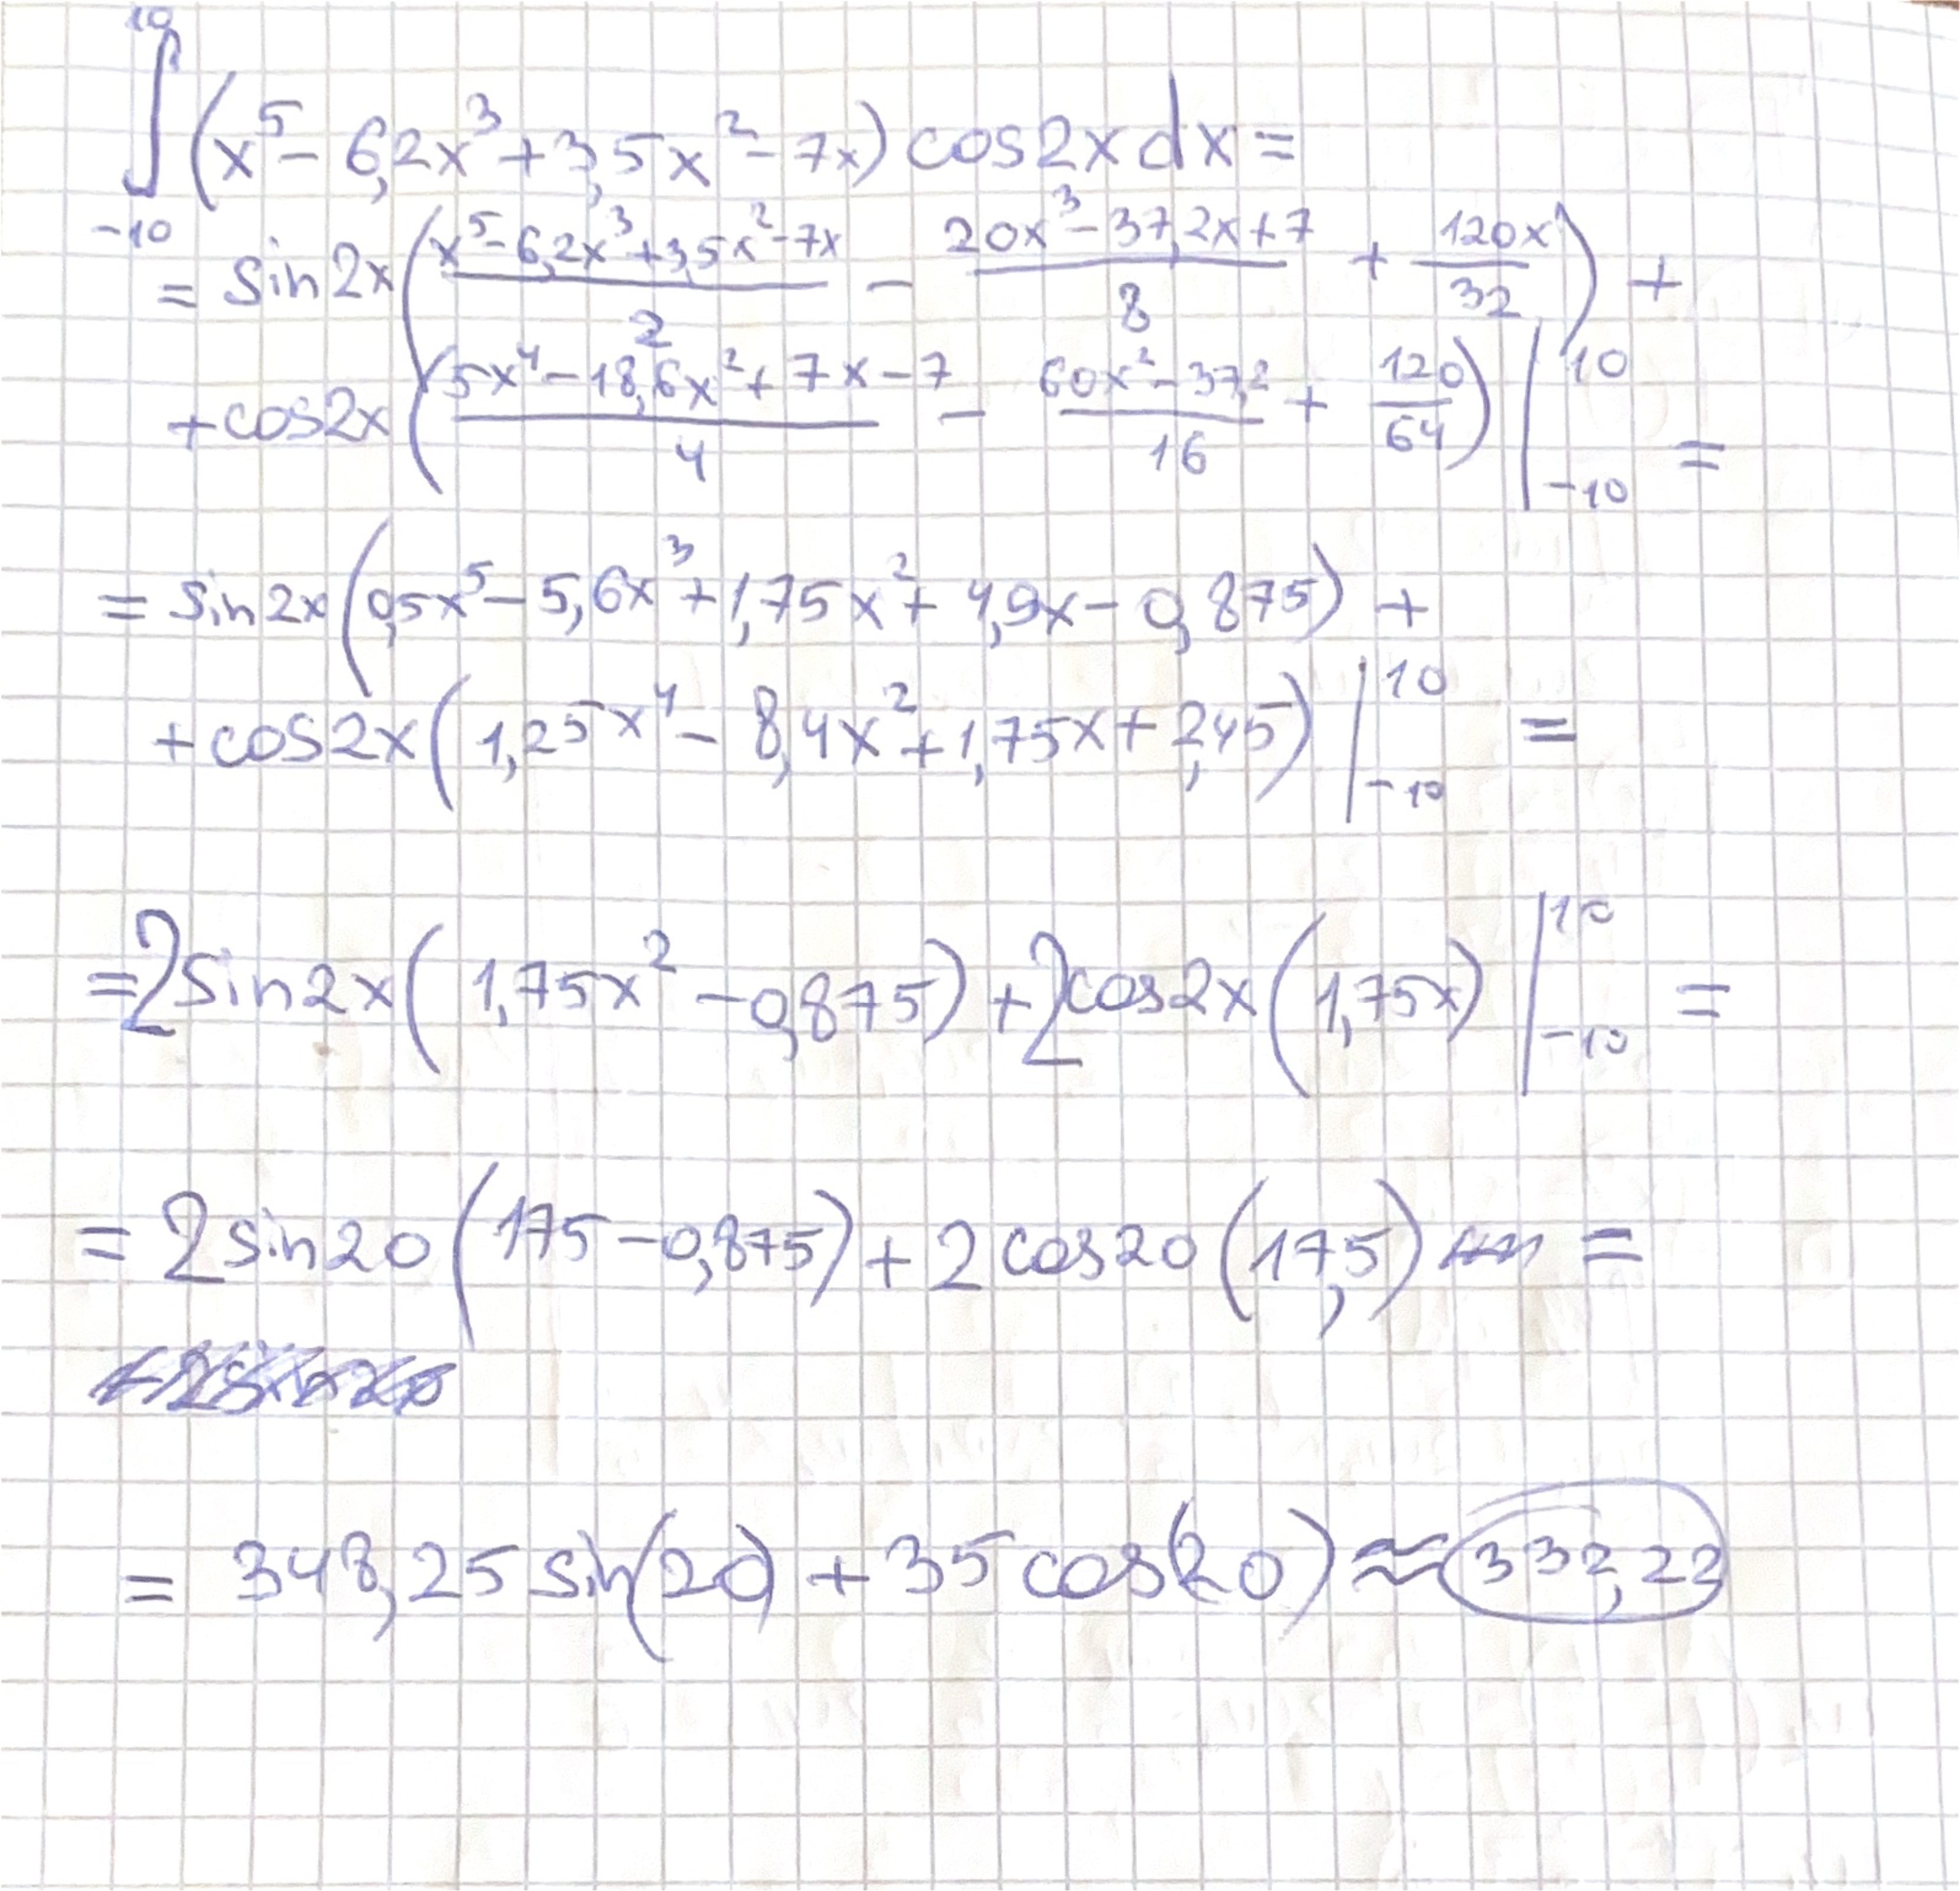
\includegraphics[width=0.9\linewidth]{../data/calculation.pdf}
			\caption{Подсчет интеграла}
			\label{fig:calculation}
		\end{framed}
	\end{figure}
	
	\begin{figure}[H]
		\centering
		\begin{framed}
			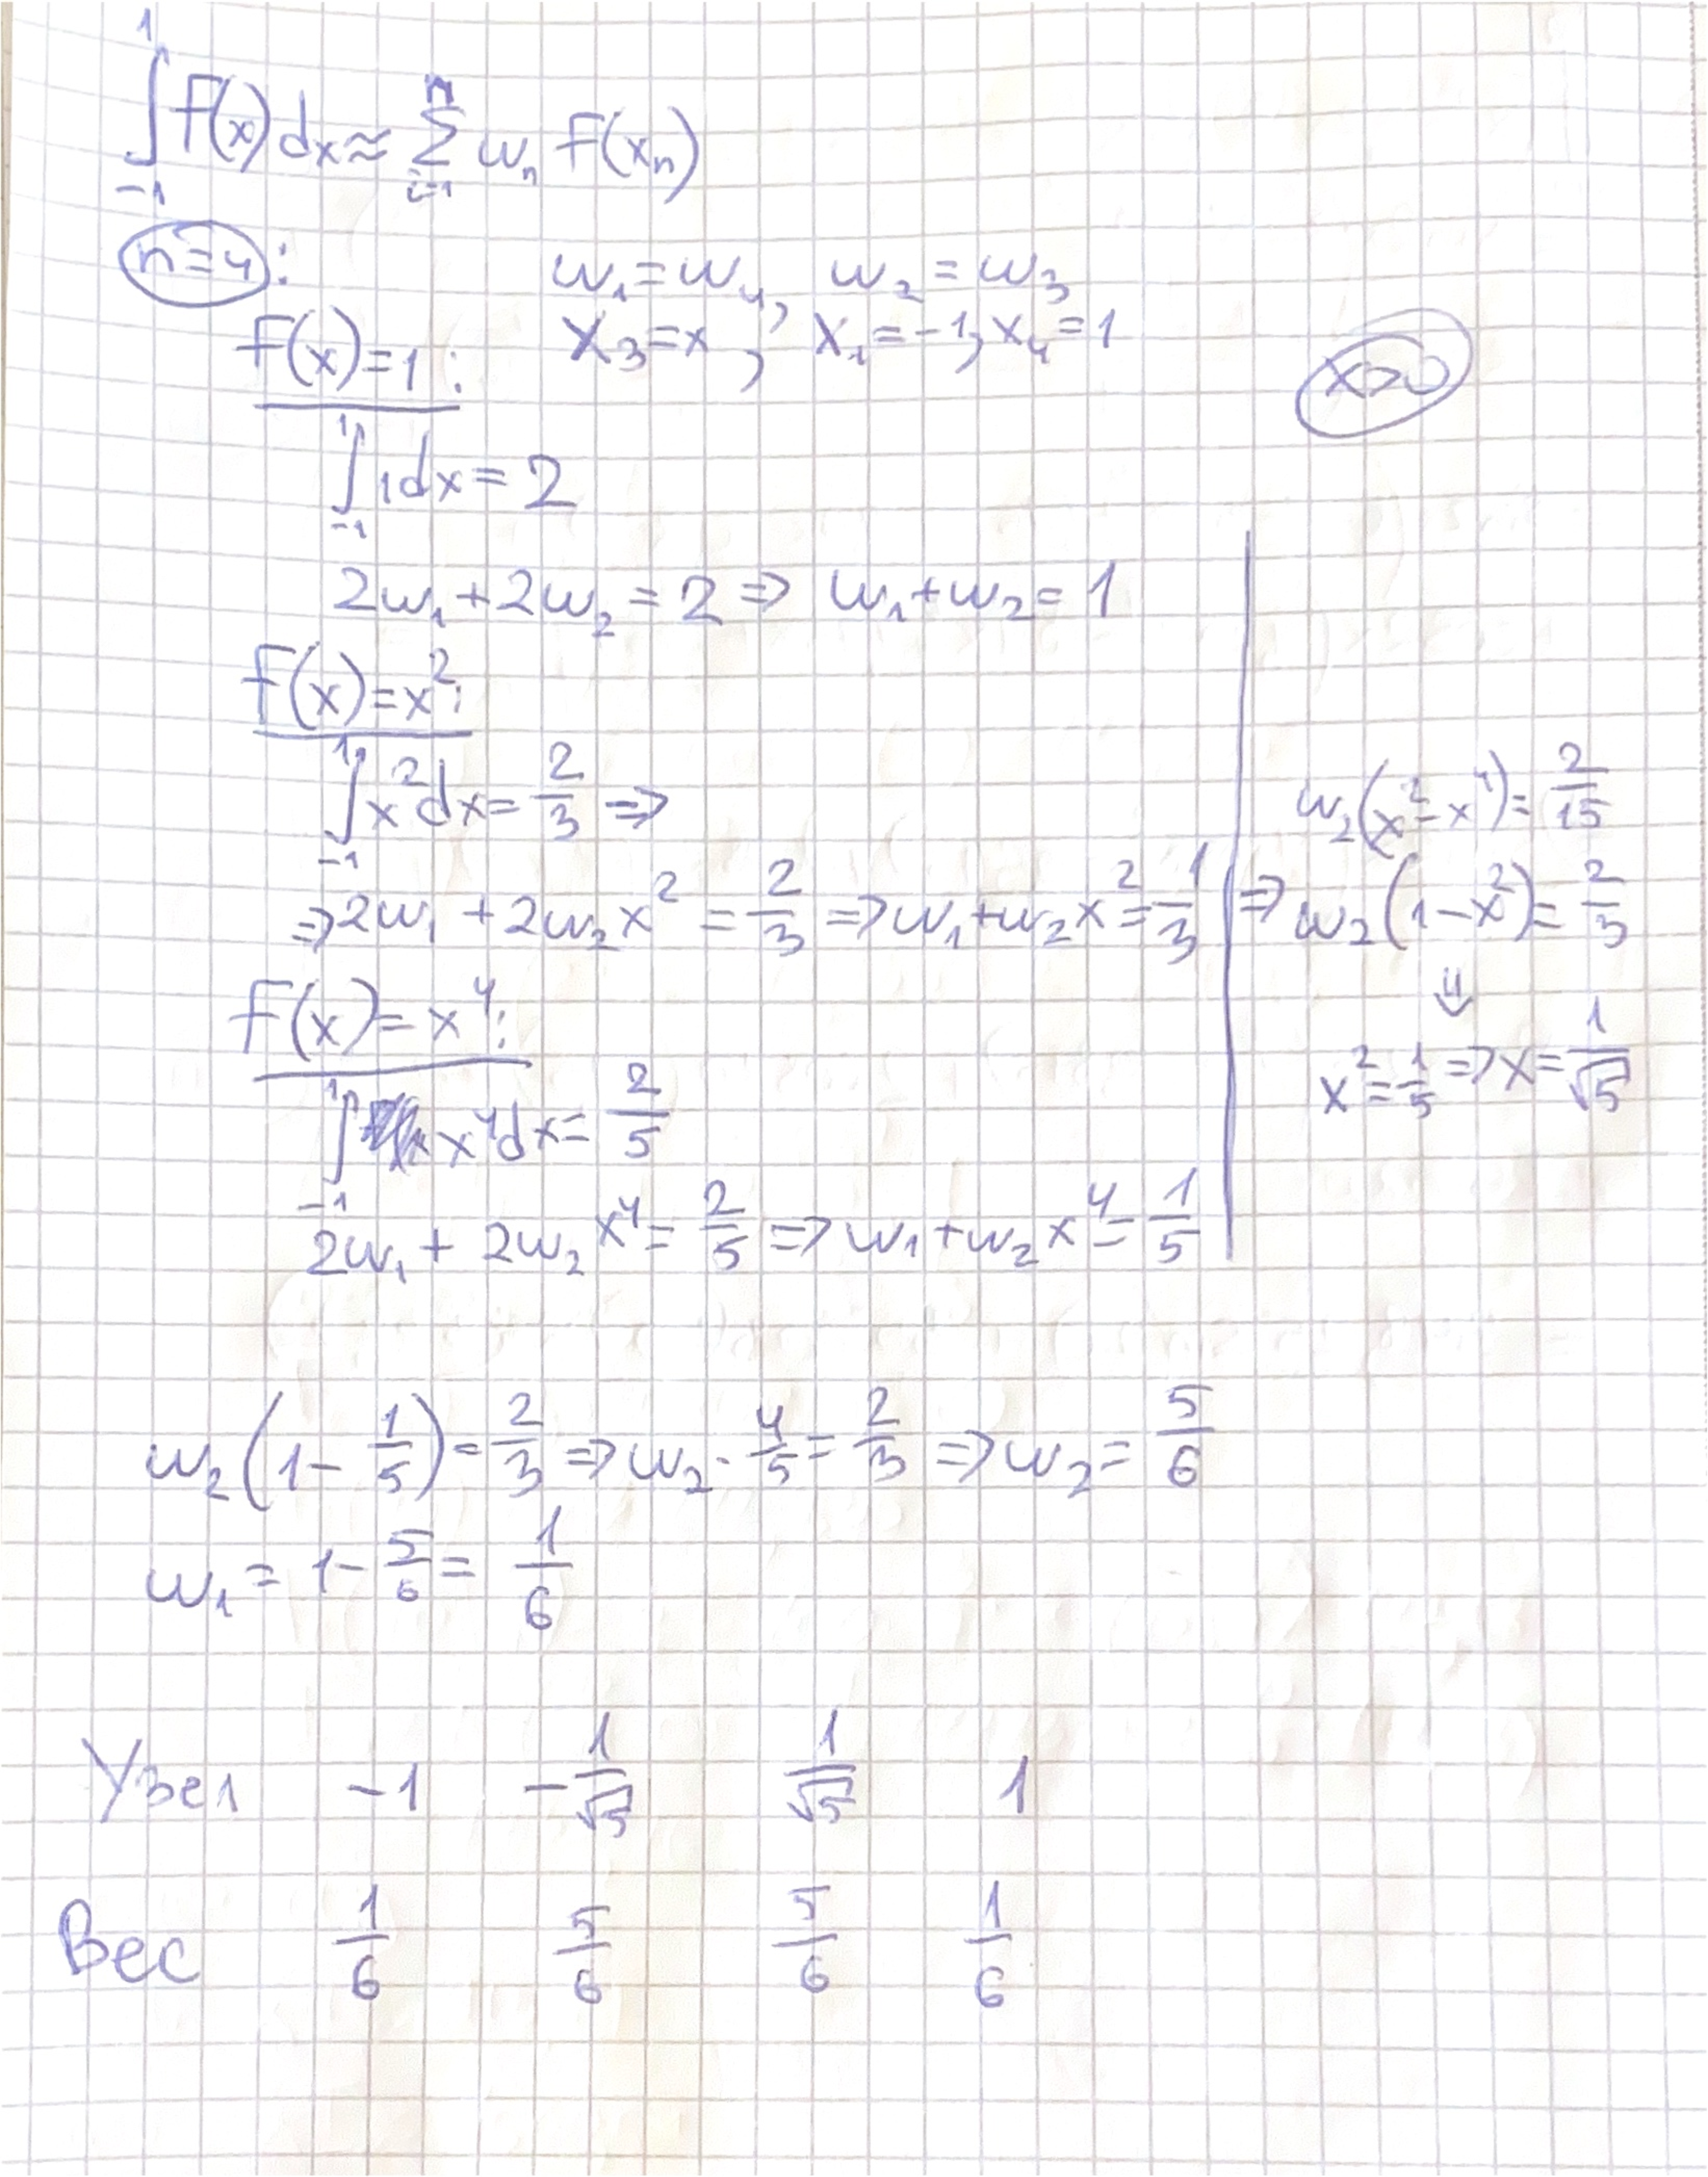
\includegraphics[width=0.9\linewidth]{../data/prior_analysis_1.pdf}
			\caption{Предварительный анализ (страница 1)}
			\label{fig:prior_1}
		\end{framed}
	\end{figure}
	
	\begin{figure}[H]
		\centering
		\begin{framed}
			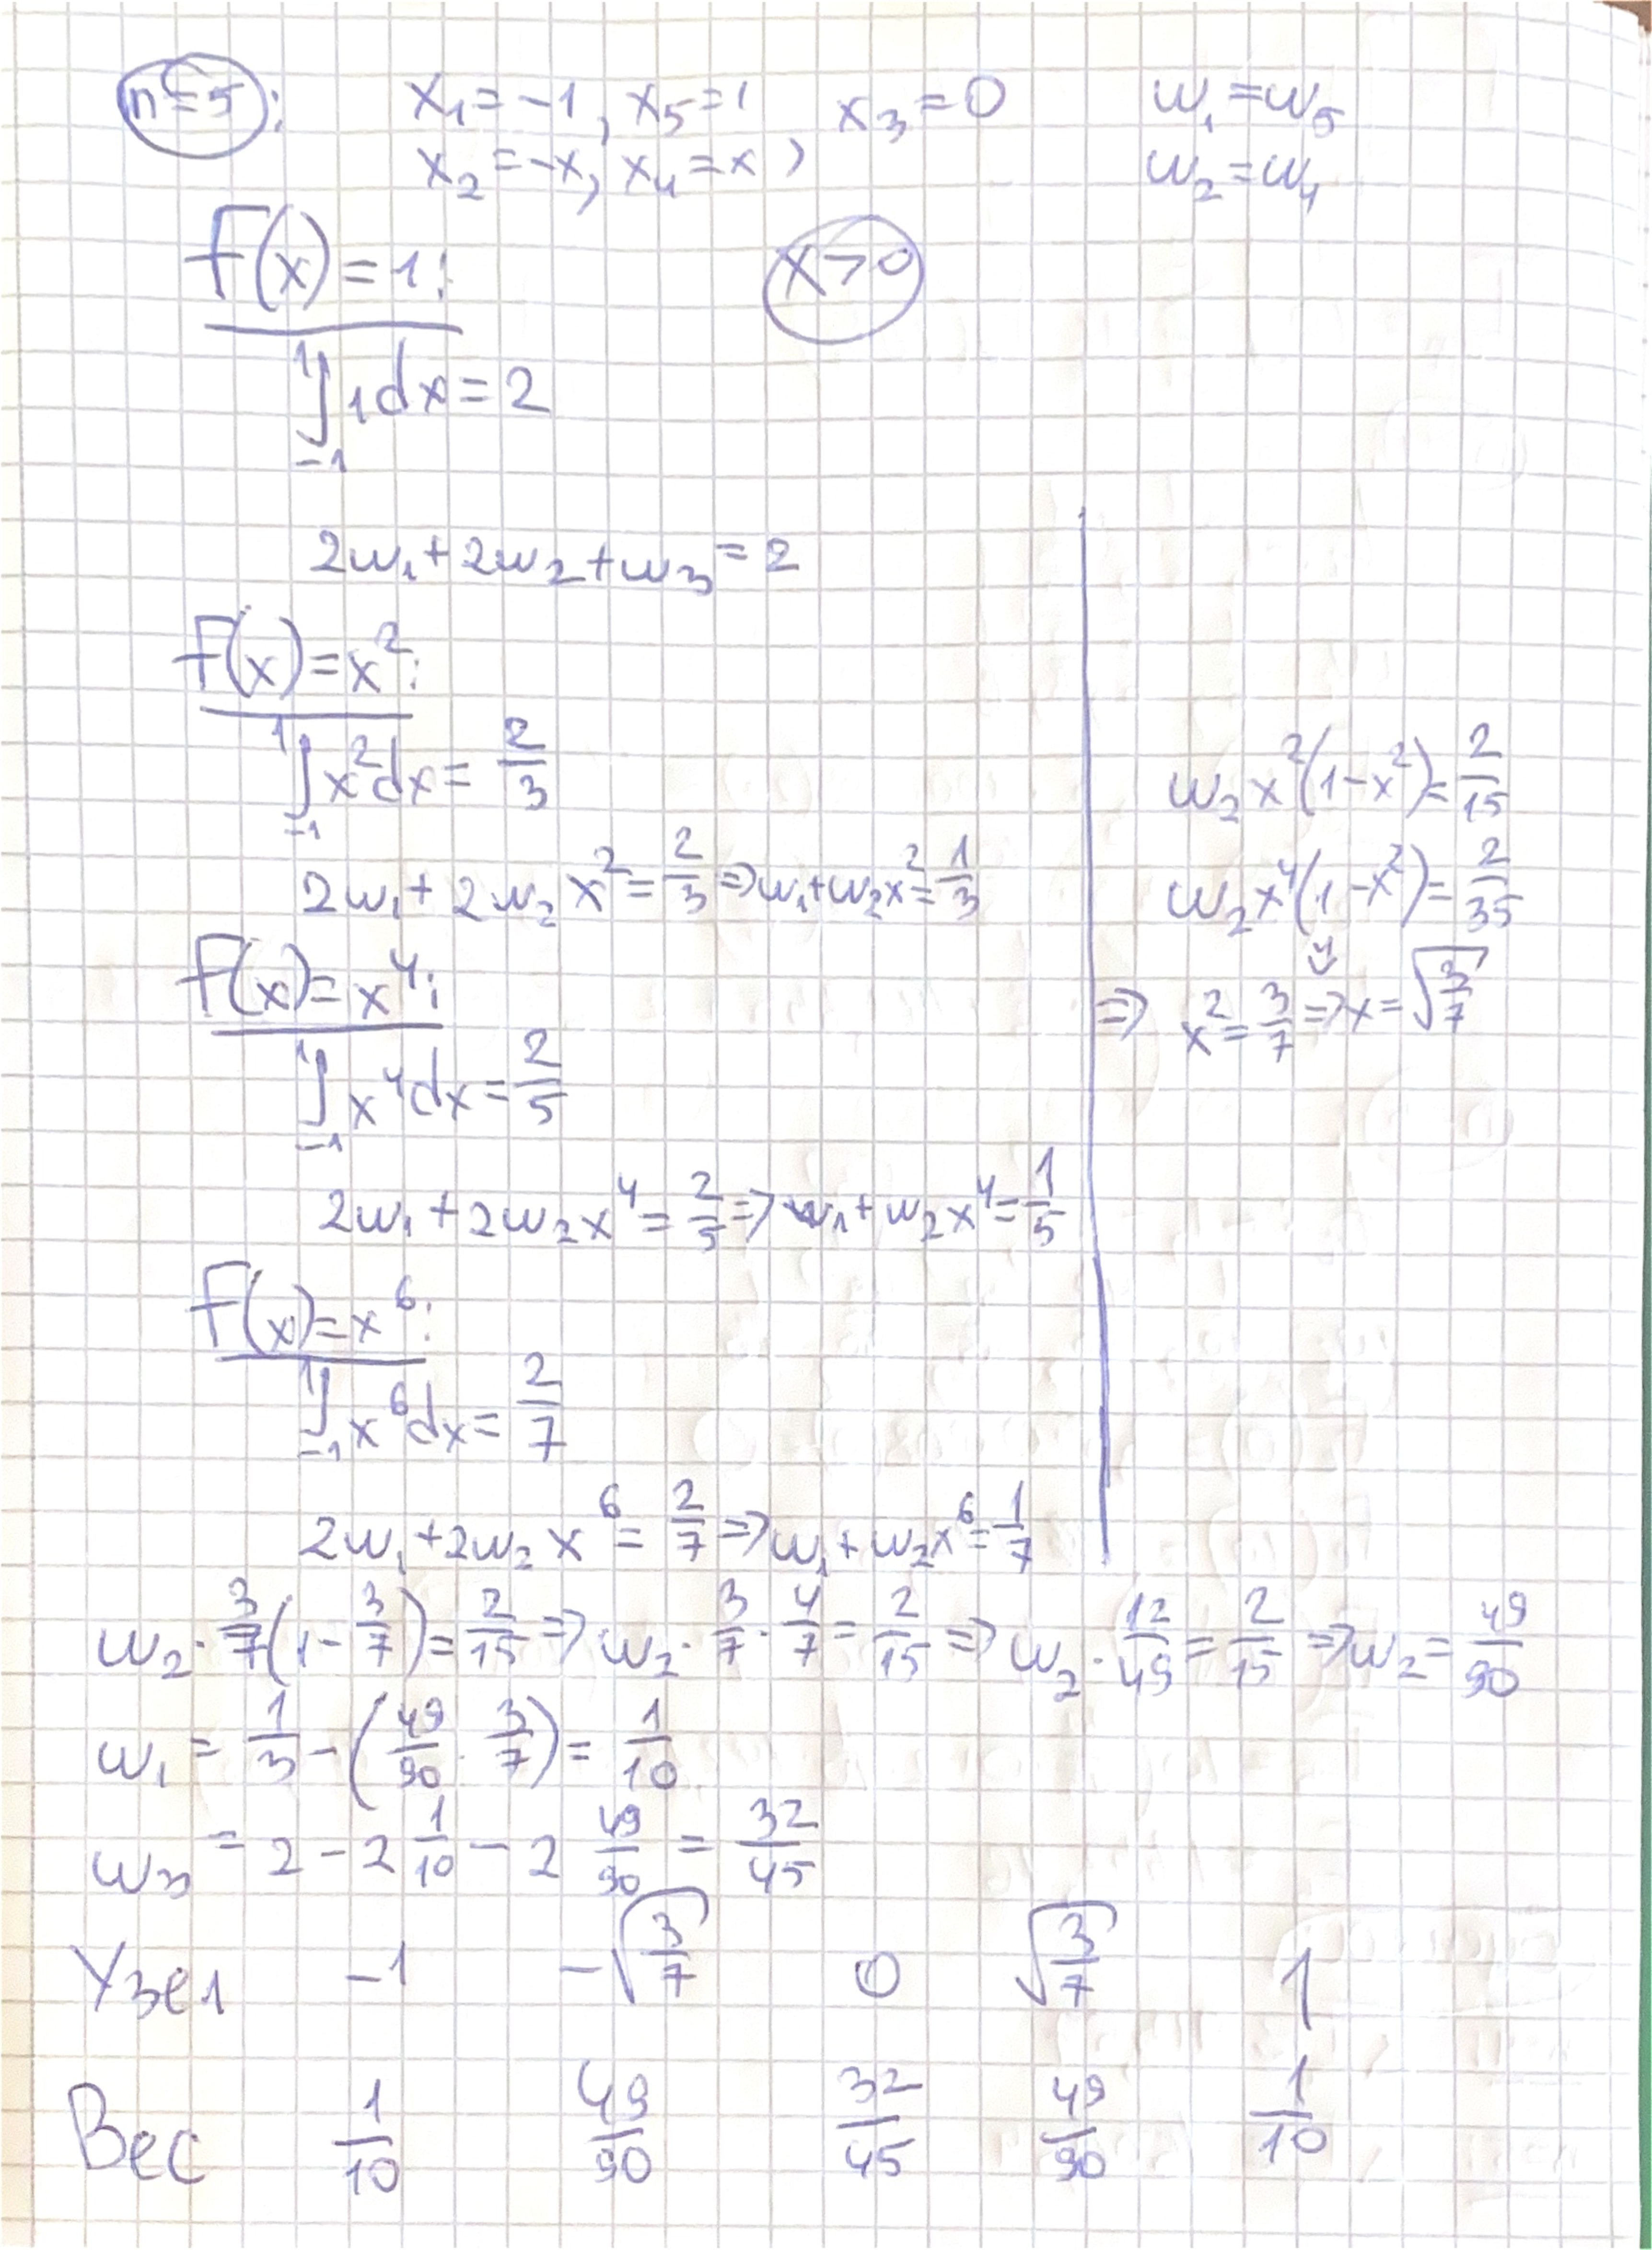
\includegraphics[width=0.9\linewidth]{../data/prior_analysis_2.pdf}
			\caption{Предварительный анализ (страница 2)}
			\label{fig:prior_2}
		\end{framed}
	\end{figure}
	
	%-------- the fourth point --------
	
	\newpage
	\section{\Large \underline{Тестовый пример}}
	
	\begin{figure}[H]
		\centering
		\begin{framed}
			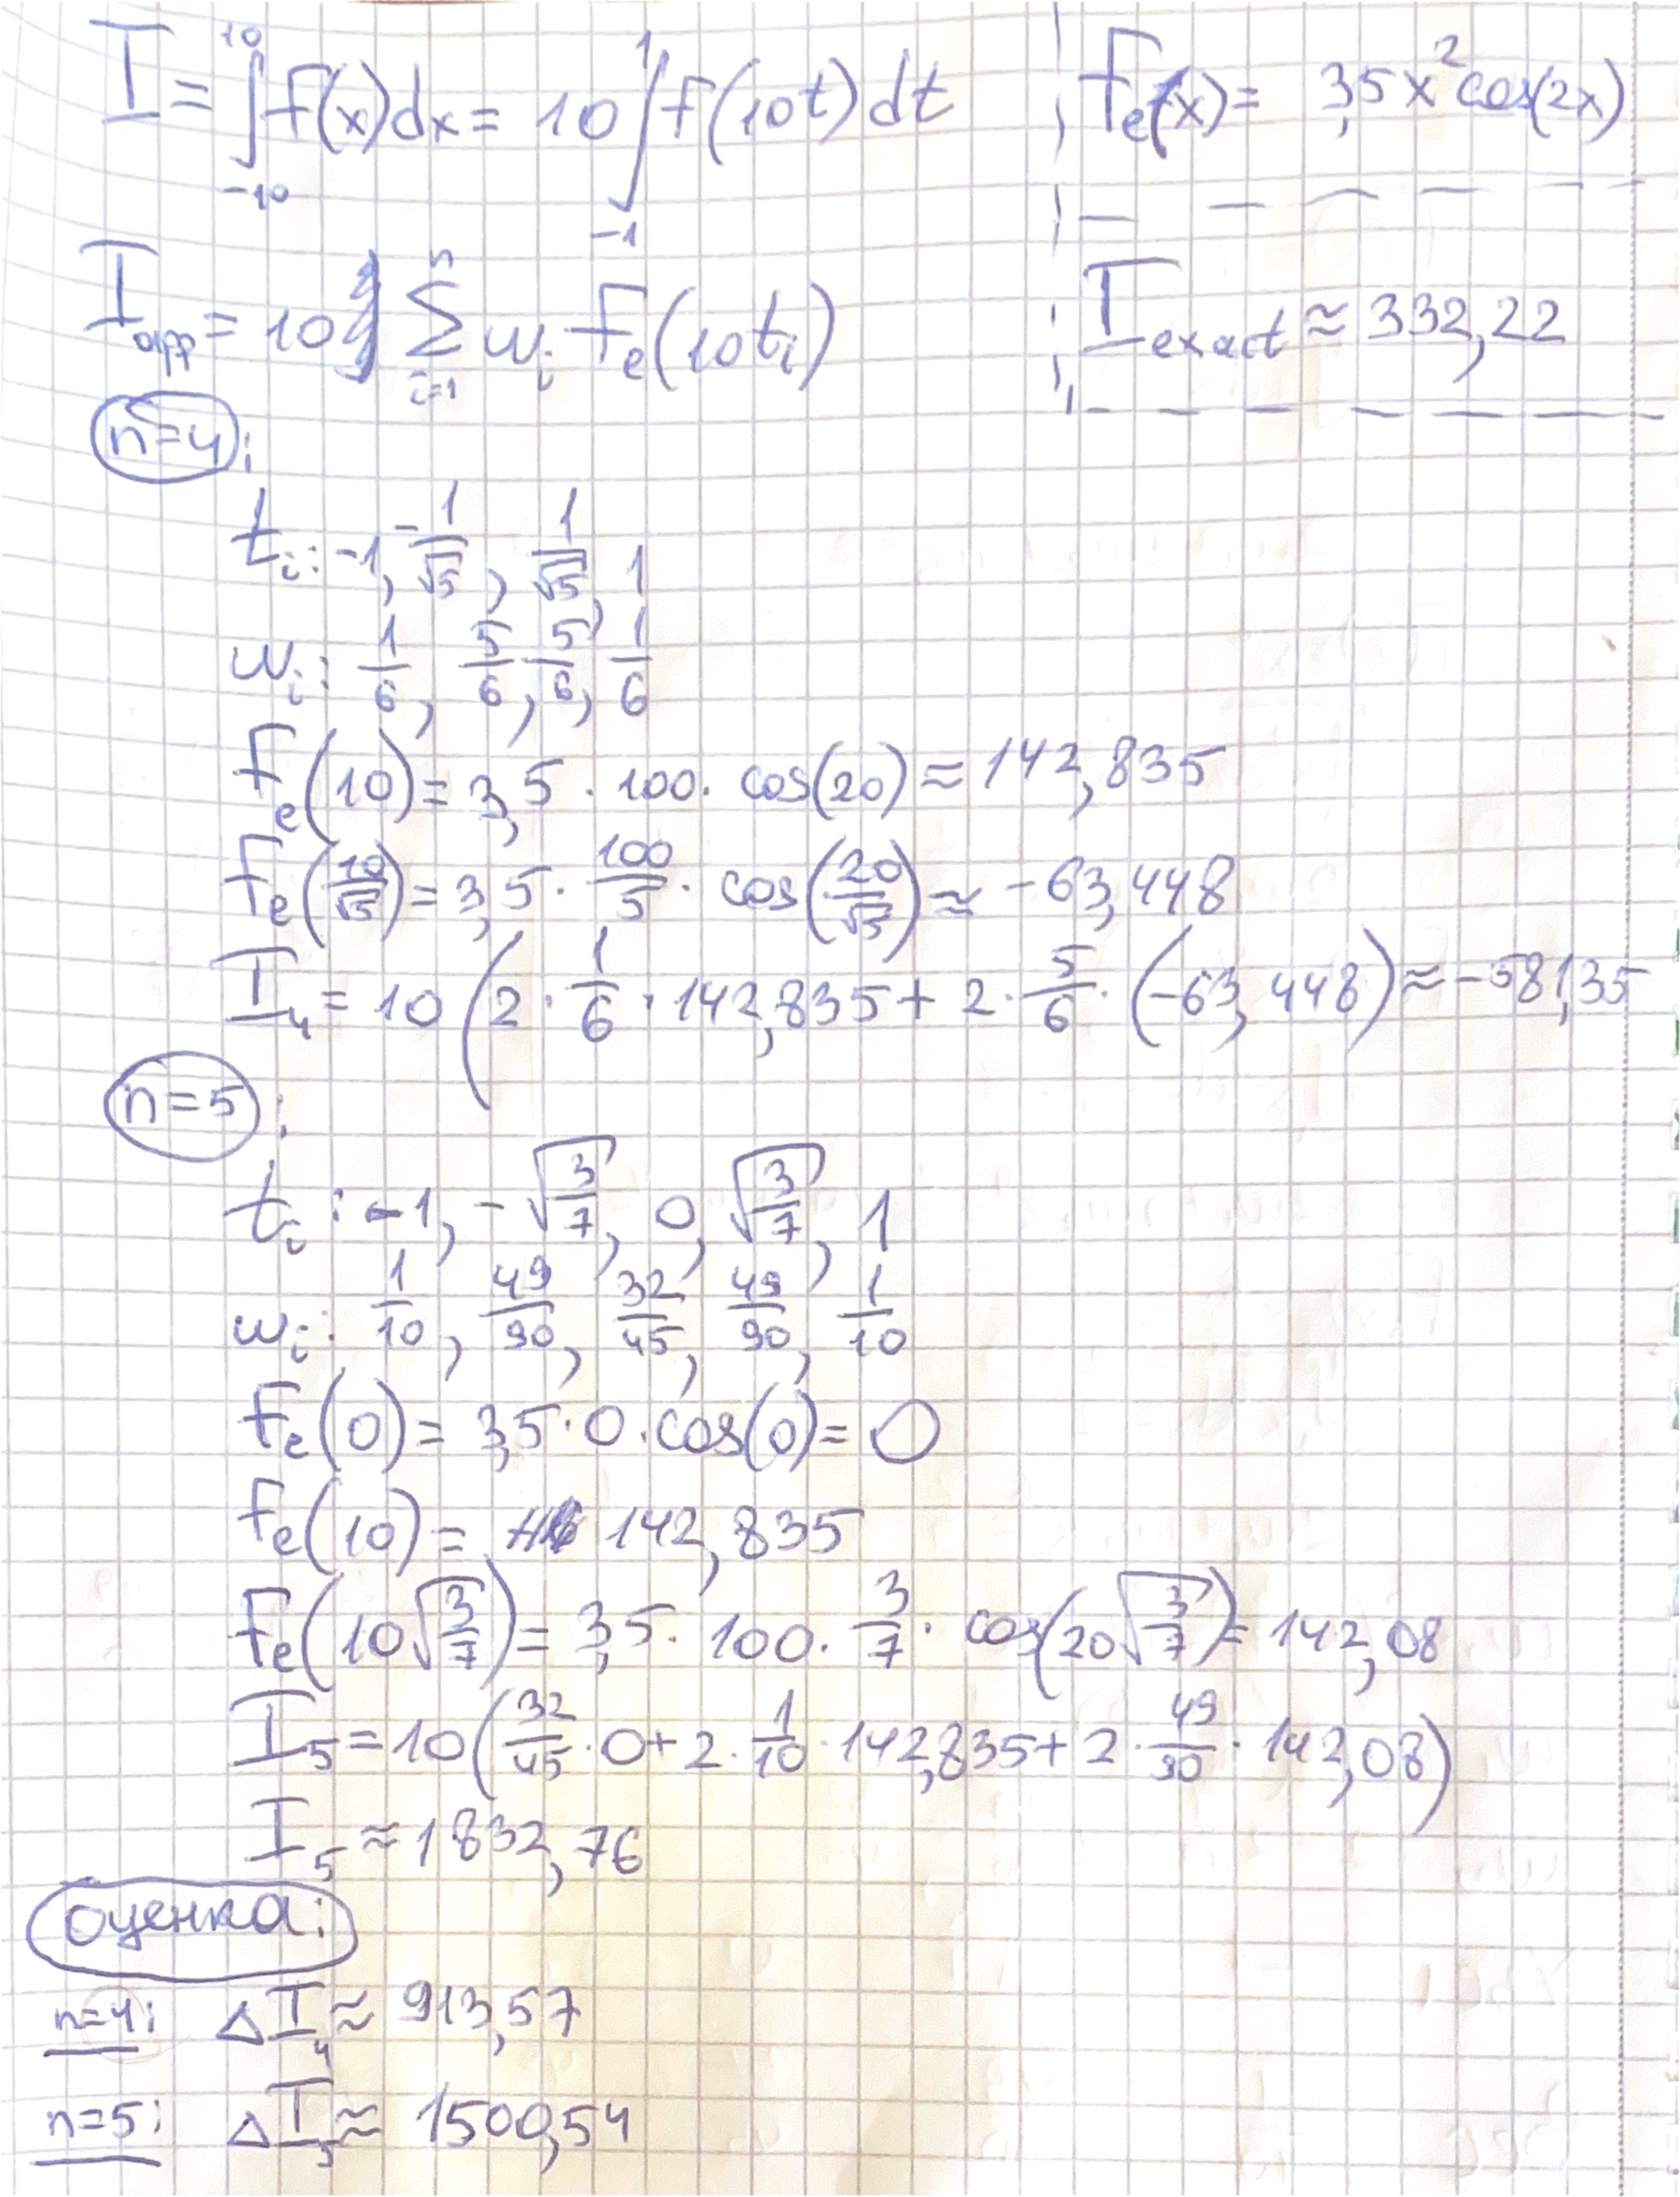
\includegraphics[width=0.9\linewidth]{../data/test_example.pdf}
			\caption{Тестовый пример}
			\label{fig:test}
		\end{framed}
	\end{figure}
	
	\newpage
	
	При сопоставлении результатов глобальных квадратурных формул Лобатто для $n=4$ и $n=5$ обнаружено катастрофическое расхождение значений ($-581.35$ и $1832.76$ соответственно) с точным значением интеграла ($\approx 332.22$).Данный феномен не является следствием вычислительной ошибки, а представляет собой классическую проблему недостаточной дискретизации быстроосциллирующих функций. Поскольку период функции $\cos(2x)$ равен $T = \pi \approx 3.14$, на интервале $[-10, 10]$ укладывается более 6 полных периодов.При $n=4$ узлы распределены так, что внутренние узлы попадают на отрицательные полуволны функции, из-за чего интерполирующий полином искусственно занижает значение интеграла.При $n=5$ узлы смещаются и попадают исключительно на пики положительных полуволн, из-за чего метод аппроксимирует знакопеременную функцию как строго положительную.
	
	\begin{figure}[H]
		\centering
		\begin{framed}
			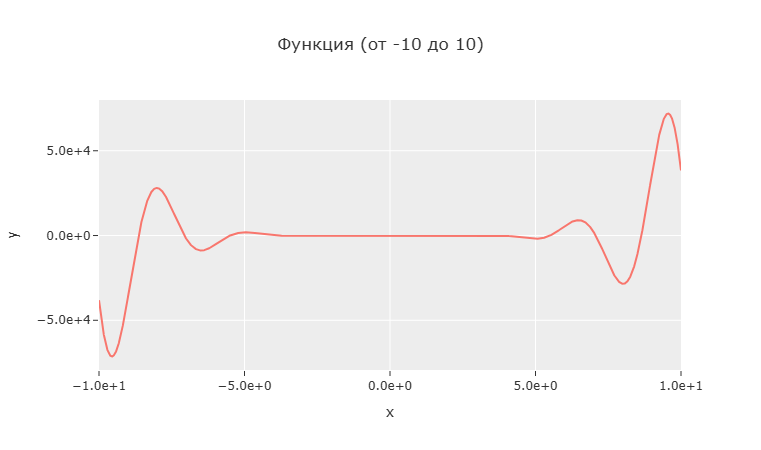
\includegraphics[width=0.9\linewidth]{../data/func_full.png}
			\caption{Тестовая функция}
			\label{fig:func_full}
		\end{framed}
	\end{figure}
	
	\begin{figure}[H]
		\centering
		\begin{framed}
			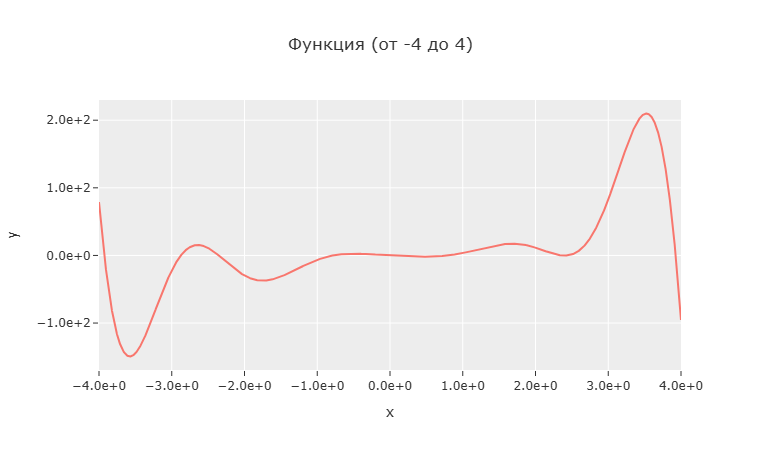
\includegraphics[width=0.9\linewidth]{../data/func_part.png}
			\caption{Тестовая функция (от -4 до 4)}
			\label{fig:func_part}
		\end{framed}
	\end{figure}

	
	
	%-------- the fifth point --------
	
	\newpage
	\section{\Large \underline{Подготовка контрольных тестов}}
	
	В качестве тестовой функции используется:
	\[
	f(x) = (x^5 - 6.2x^3 + 3.5x^2 - 7x)\cdot \cos(2x).
	\]
	
	Рассматриваемый интеграл:
	\[
	I = \int\limits_a^b f(x)\,dx.
	\]
	
	Точное значение интеграла вычисляется аналитически.
	
	Контроль проводится:
	\begin{itemize}
		\item сравнением численного и точного значений;
		\item анализом зависимости ошибки от параметров метода;
		\item исследованием сходимости.
	\end{itemize}
	
	%-------- the sixth point --------
	
	\section{\Large \underline{Модульная структура программы}}
	
	\begin{itemize}
		\item \textbf{function} — вычисление функции $f(x)$
		\begin{itemize}
			\item вход: $x$
			\item выход: $f(x)$
		\end{itemize}
		
		\item \textbf{lobatto\_4 / lobatto\_5} — квадратурные формулы Лобатто
		\begin{itemize}
			\item вход: $a, b$
			\item выход: значение интеграла на отрезке
		\end{itemize}
		
		\item \textbf{adaptive\_integrate} — адаптивное разбиение
		\begin{itemize}
			\item вход: $a, b, \varepsilon$
			\item выход: значение интеграла, число разбиений
		\end{itemize}
		
		\item \textbf{richardson} — уточнение результата
		\begin{itemize}
			\item вход: два приближения, порядок метода
			\item выход: уточнённое значение
		\end{itemize}
	\end{itemize}
	
	%-------- the eighth point --------
	
	\newpage
	\section{\Large \underline{Численный анализ решения задачи}}
	
	\begin{enumerate}[label*=\arabic*), align=left, leftmargin=*, itemindent=1.5em, listparindent=1.5em, parsep=0pt]
		\begin{figure}[H]
			\centering
			\begin{framed}
				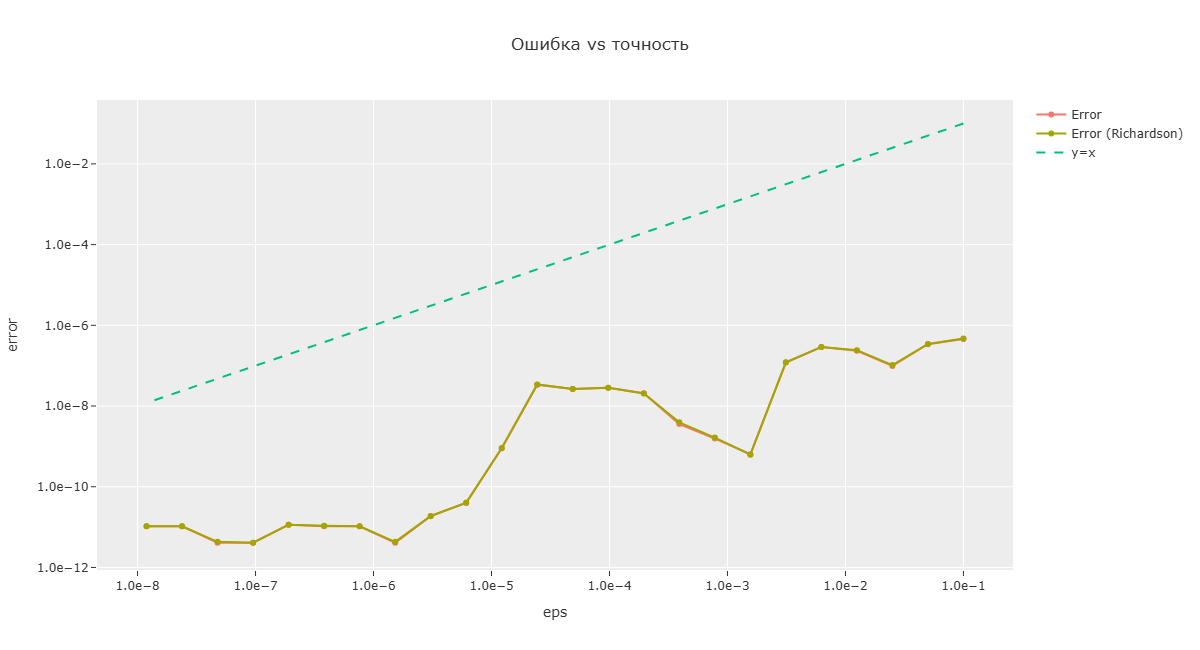
\includegraphics[width=0.9\linewidth]{../data/error_eps.png}
				\caption{График зависимости ошибки от заданной точности}
				\label{fig:error_eps}
			\end{framed}
		\end{figure}
		
		\begin{figure}[H]
			\centering
			\begin{framed}
				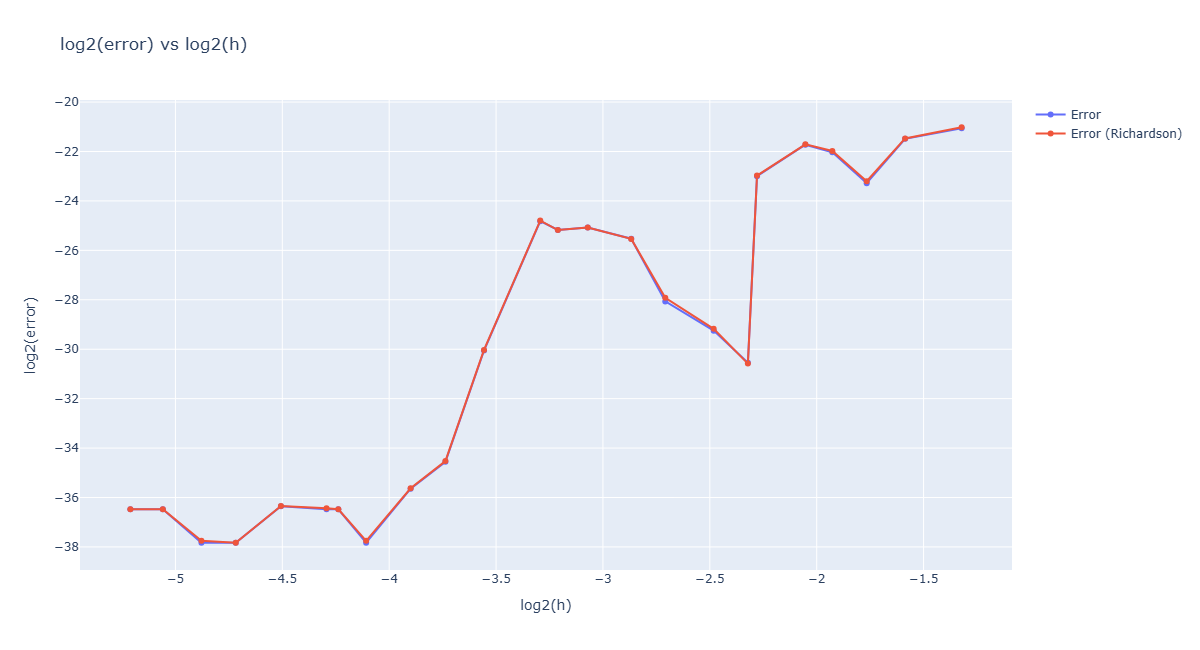
\includegraphics[width=0.9\linewidth]{../data/error_h.png}
				\caption{График зависимости ошибки от длины отрезка разбиения}
				\label{fig:error_h}
			\end{framed}
		\end{figure}

		
		\newpage
		\item Построен график зависимости ошибки от заданной точности \eqref{fig:error_eps}.
		
		При уменьшении точности ошибка падает. Причем построенная биссектриса говорит о том, что метод достигает заданной точности
		
		\item Далее был построен график зависимости ошибки от длины отрезка разбиения в логарифмическом масштабе \eqref{fig:error_h} 
		
		Меньшее разбиение дает меньшую ошибку.
		
		По графику были определены порядок точности: $p \approx 6.1$
		
		а также константа: $C \approx 5.7 \cdot 10^{-7}ы$ 
		
	\end{enumerate}
	
	
	
	%-------- the ninth point --------
	
	\newpage
	\section{\Large \underline{Выводы}}

	В работе был реализован численный метод вычисления определённого интеграла с использованием квадратурных формул Гаусса–Лобатто.
	
	Была обеспечена заданная точность вычислений с применением адаптивного разбиения. Проведён анализ погрешности метода и подтверждён его порядок точности.
	
	Результаты численного анализа согласуются с теоретическими оценками.
	
	
\end{document}